\documentclass[utf8]{article}

%\usepackage{doi}
\usepackage{authblk}
\usepackage[T1]{fontenc}
\usepackage[utf8]{inputenc}
\usepackage[pdftex]{xcolor}
\usepackage[pdftex]{graphicx}
\usepackage[authoryear,round]{natbib}

% review mode
\usepackage{geometry}
\usepackage{lineno}
\linenumbers
\linespread{1.5}

% custom colours
\definecolor{darkblue}{cmyk}{0.9,0.3,0.0,0.0}
\definecolor{darkgreen}{cmyk}{0.8,0.0,1.0,0.0}
\definecolor{darkred}{cmyk}{0.1,0.9,0.8,0.0}
\definecolor{darkorange}{cmyk}{0.0,0.5,1.0,0.0}
\definecolor{darkpurple}{cmyk}{0.6,0.7,0.0,0.0}
\definecolor{darkbrown}{cmyk}{0.23,0.73,0.98,0.12}

% custom commands
\newcommand{\idea}[1]{\textcolor{darkgreen}{\emph{[\textbf{IDEA:} #1]}}}
\newcommand{\note}[1]{\textcolor{darkblue}{\emph{[\textbf{NOTE:} #1]}}}
\newcommand{\todo}[1]{\textcolor{darkred}{\emph{[\textbf{TODO:} #1]}}}
\newcommand{\aref}[0]{\textcolor{darkblue}{\textbf{[REF.]}}}
\newcommand{\ian}[1]{\textcolor{darkbrown}{\emph{[\textbf{IAN:} #1]}}}

\graphicspath{{../../figures/}}

\title{Last glacial cycle glacier erosion potential in the Alps}
\author[1]{Julien Seguinot}
\author[2]{Ian Delaney}
\affil[1]{Anafi, Greece} % {\small (juseg \emph{at} posteo.eu)}}
\affil[2]{Institute of Earth Surface Dynamics, University of Lausanne, Switzerland}


% ======================================================================
\begin{document}
% ======================================================================

\maketitle

\begin{abstract}

    The glacial landscape of the Alps has fascinated generations of explorers,
    artists, mountaineers and scientists with its diversity, including
    erosional features of all scales from high-mountain cirques, to steep
    glacial valleys and large over-deepened basins. Using previous glacier
    modelling results, and empirical inferences bedrock erosion under modern
    glaciers, we compute a distribution of potential glacier erosion in the Alps
    over the last glacial cycle from 120\,000 years ago to the present.
    %
    Despite large uncertainties related to the climate history of the Alps and
    unconstrained glacier erosion processes, the resulting modelled patterns of
    glacier erosion shows persistent features. The cumulative imprint of
    the last glacial cycle shows a very strong localization of glacier erosion
    with local maxima at the mouths of major Alpine valleys and some other
    upstream sections where glaciers are modelled to have flown with the
    highest velocity. The modelled erosion rates vary significantly through the
    glacial cycle, but show paradoxically little relation to the glaciation
    extent. Phases of glacier advance and maximum extension, characterized by
    low air and glacier temperatures, see a localization of rapid erosion rates
    at low elevation, while intra-montane areas are modelled to date from phases
    of intermediate glacier cover. The modelled erosion rates peak during
    deglaciation phases, when higher air and glacier temperature enhance
    glacier dynamics.
    %
    Our results depict the Alpine glacier erosion landscape as a
    time-transgressive patchwork, with different erosional landscapes of the
    same mountain range corresponding to different glaciation stages and time
    periods, thus offering insight into its diversity.

\end{abstract}


% ----------------------------------------------------------------------
\section{Introduction}
% ----------------------------------------------------------------------

    The glacial erosion landscape of the Alps has fascinated generations of
    explorers, artists, mountaineers and scientists for centuries. Its cultural
    impact is indeed so far-reaching, that in English, a non-Alpine language,
    the adjective ``alpine'' with non-capital ``a'' is now casually used to
    describe an Alpine-like, glacially modified mountain landscape outside the
    Alps, while the proper noun ``Alps'' has been applied to nick-name
    Alpine-like, glacier eroded mountain ranges in Norway (\emph{Lyngsalpene}),
    New Zealand (Southern Alps), Japan (\emph{Nihon Arupusu}), and elsewhere.

    Some mountain ranges are predominantly characterised by cirque glaciation
    (e.g. Uinta Mountains), glacial valleys (e.g. Putorana Plateau), or
    large-scale overdeepenings (e.g. Patagonia). But other regions, including
    the Alps, present a higher variety glacial erosional landforms
    (Fig.~\ref{fig:landscape}), whose implications on glacial history is yet to
    be understood.

    In absence of other glacial landforms, the degree of glacial modification
    of a landscape has sometimes been used as a proxy for the duration of past
    glacier cover, as for instance in geomorphological mapping \aref. However,
    cold-based glaciers have been shown to preserve landforms as fragile as
    sand beaches \aref. Yet it remains unclear how sharp the erosional
    transition to cold-based ice is, and why some glaciated regions show
    glacially preserved landscapes and others, including the Alps, do not
    \aref.

    While it has long been understood that glaciers leave a specific erosional
    imprint on the landscape, observing and quantifying the long-term erosion
    and sedimentation processes has been a challenge, not least due to the
    inaccessibility of glacier beds and the slow and stochastic nature of
    glacial erosion processes \aref. \ian{Perhaps this needs more detail?}

    More recent studies have moved away from process
    understanding towards attempts at calibrating empirical erosion laws for an entire
    glacier or set of glaciers. \citet{Koppes.etal.2015} quantified sediment
    yields in 15~Patagonian and Antarctic Peninsula fjords, concluding at a
    predominant control of surface air temperature on rapid glacier erosion and
    calibrating a near-square-law from glacier velocity to erosion rate.
    \citet{Herman.etal.2015} collected suspended sediment samples for 5~months
    in the outlet stream of Franz-Josef Glacier, mapped their chemical
    composition to geologic zones of distinctive glacier speed, and also
    concluded to a near-square relationship between basal sliding and glacier
    erosion, but yielding much higher erosion rates.
    \citet{Cook.etal.2020} assembled a global compilation of erosion rates for
    38~glaciers, showing a predominant role of glacier sliding velocity over
    climate variables, yet concluding at a sub-linear relationship to erosion.

    Here, the non-linear erosion law by \citet{Koppes.etal.2015} is applied to
    previously published model results \citep{Seguinot.etal.2018} and the
    patterns of modelled erosion rate and cumulative last glacial cycle erosion
    potential are analysed. Despite aggregated uncertainties on paleoclimate,
    glacier flow and glacier erosion processes, out results provide insights
    into the diversity of the Alpine glacial erosion landscape.


% ----------------------------------------------------------------------
\section{Methods}
% ----------------------------------------------------------------------

% -- -- -- -- -- -- -- -- -- -- -- -- -- -- -- -- -- -- -- -- -- -- -- -
\subsection{Ice sheet modelling}
% -- -- -- -- -- -- -- -- -- -- -- -- -- -- -- -- -- -- -- -- -- -- -- -

    The ice-sheet model set-up was presented, and the results discussed, in an
    earlier publication \citep{Seguinot.etal.2018}. The simulations use the
    Parallel Ice Sheet Model (PISM, development version~e9d2d1f), an open
    source, finite difference, shallow ice sheet model
    \citep{PISM-authors.2017}. The model includes temperature and water-content
    dependent creep, pseudo-plastic basal sliding accounting for till
    dilatation under high water pressure, bedrock deformation under the ice
    load, and a~positive degree-day (PDD) surface mass balance model. The model
    is initialized with assumed present-day ice thickness and equilibrium
    ice and bedrock temperature at 120\,ka, and ran to the present.
    Climate forcing is provided by a~monthly climatology from interpolated
    observational data \citep[WorldClim;][]{Hijmans.etal.2005} and the European
    Centre for Medium-Range Weather Forecasts Reanalysis Interim
    \citep[ERA-Interim;][]{Dee.etal.2011}, amended with temperature lapse-rate
    corrections from the European Project for Ice Coring in Antarctica
    \citep[EPICA;][] {Jouzel.etal.2007}, and in some cases, time-dependent
    palaeo-precipitation reductions. Lower-resolution, alternative climate
    scenarios are analyzed in the discussion part
    (Sect.~\ref{sec:sensitivity}).

    Physical parametres are listed in the earlier open-access publication
    \citep{Seguinot.etal.2018} and complete PISM set-up is stored in long-term
    archived model output metadata for this \todo{DOI}, and for the earlier
    \todo{DOIs} publications.

% -- -- -- -- -- -- -- -- -- -- -- -- -- -- -- -- -- -- -- -- -- -- -- -
\subsection{Erosion law}
% -- -- -- -- -- -- -- -- -- -- -- -- -- -- -- -- -- -- -- -- -- -- -- -

    Modelled erosion rates, $\dot{e}$, are calculated from the modelled basal
    velocities, $u_\mathrm{b}$, using a empirical erosion power-law,
    %
    \begin{equation}
        \dot{e} = K_\mathrm{g} u_\mathrm{b}^l ,
    \end{equation}
    %
    where $K_g = 5.2\times 10^{-11}\,m^{1-l}\,a^{l-1}$ and $l = 2.34$ are
    empirical constants calibrated on quantified sediment yields and velocities
    from 15~Patagonian and Antarctic Peninsula tidewater glaciers
    \citep{Koppes.etal.2015}. It is important to note that there are both large
    uncertainties surrounding these numbers on the aforementioned glaciers
    \todo{quantify}, and little insurance that this erosion law applies
    elsewhere. Alternative erosion laws are analyzed in the discussion part
    (Sect.~\ref{sec:powerlaws}).

    \note{I initially built the paper around the erosion law by
          \citep{Herman.etal.2015}, that yielded similar erosion patterns but
          up to several km of cumulative erosion in the valleys.}

    Unlike landscape evolution model studies \aref, this study does not account
    for the feedback of glacier erosion onto bedrock topography and ice dynamics.
    Neither are other forms of erosion accounted for. Instead, the
    time-integrated erosion rate,
    %
    \begin{equation}
        e =  K_\mathrm{g} \int u_\mathrm{b}^l dt,
    \end{equation}
    %
    is later referred to as the cumulative ``erosion potential''. This erosion
    potential is numerically approximated using a time-step of 10\,a in the
    main simulation, and 100\,a in the alternative climate scenarios runs. It
    can already be noticed from the above formula, that with an exponent, $l$,
    higher than one, the cumulative erosion potential has a greater dependency
    on the basal ice dynamics, $u_\mathrm{b}$, than the timing of glacier
    cover, $dt$.


% ----------------------------------------------------------------------
\section{Results}
% ----------------------------------------------------------------------

% -- -- -- -- -- -- -- -- -- -- -- -- -- -- -- -- -- -- -- -- -- -- -- -
\subsection{Cumulative erosion}
% -- -- -- -- -- -- -- -- -- -- -- -- -- -- -- -- -- -- -- -- -- -- -- -

    The modelled cumulative (time-integrated) glacial erosion potential
    (Fig.~\ref{fig:cumulative}a) varies by several orders of magnitude
    from insignificant to hundred-metres scale erosion
    potential. Its spatial patterns show a very
    strong localization along the Alpine valleys, with local maxima occuring both at
    the Alpine gates where ice flow transited from valley to piedmont glaciers,
    and further up-valley where valley slopes increase.
    There is a genereral tendency for higher cumulative erosion in the
    north-western Alps where the input winter precipitation
    \citep[WorldClim,][Fig.~1h]{Seguinot.etal.2018} is higher and the
    preexisting glacial topography more pronounced.

% -- -- -- -- -- -- -- -- -- -- -- -- -- -- -- -- -- -- -- -- -- -- -- -
\subsection{Temporal evolution}
% -- -- -- -- -- -- -- -- -- -- -- -- -- -- -- -- -- -- -- -- -- -- -- -

    The modelled volumic (domain-integrated) glacial erosion rates
    (Fig.~\ref{fig:cumulative}b) do not correlate with the modelled total ice
    volume. A comparison between the modelled ice volume and the modelled
    volumic erosion rate shows no single relation between these two quantities, except
    for the onset and termination of the glacial cycle were ice volume is low
    and sliding processes unlikely to be captured by the model resolution.
    Instead, erosion is modelled to be higher by a factor 3 to 10 during
    periods of glacier retreat, than during periods of glacier advance
    (Fig.~\ref{fig:evolution}).

% -- -- -- -- -- -- -- -- -- -- -- -- -- -- -- -- -- -- -- -- -- -- -- -
\subsection{Spatial migration}
% -- -- -- -- -- -- -- -- -- -- -- -- -- -- -- -- -- -- -- -- -- -- -- -

    A closer look at the Rhine Glacier, one of the paleo-ice sheet's largest
    outlets, reveals a spatial migration of the modelled high erosion rates.
    During glacier advance and stages of extensive glaciation, the modelled
    erosion rates are moderate and restricted to low elevations, while the
    most interior parts of the Alps \citep[modelled to be
    largely-cold-based][Fig.~6c]{Seguinot.etal.2018}, experience insignificant
    erosion rates (Fig.~\ref{fig:transects}a and~d). The modelled erosion
    rates both increase and propagate inwards during periods of glacier
    retreat (Fig.~\ref{fig:transects}b, c and~d).

    These results can be generalized to the entire model domain by using
    (present-day) bedrock altitude as a proxy for along-flow distance
    (Fig.~\ref{fig:hypsogram}). Periods of modelled increasing and maximum ice
    volume corresponds to local modelled erosion rate minima, with significant
    erosion rates restricted to lower elevations. On the other hand, periods of
    modelled decreased ice volume (and area) correspond to higher local
    modelled erosion rates and a shift of significant erosion rates to
    higher-elevation areas (Fig.~\ref{fig:hypsogram}).


% ----------------------------------------------------------------------
\section{Discussion}
% ----------------------------------------------------------------------

% -- -- -- -- -- -- -- -- -- -- -- -- -- -- -- -- -- -- -- -- -- -- -- -
\subsection{Climate sensitivity}
\label{sec:sensitivity}
% -- -- -- -- -- -- -- -- -- -- -- -- -- -- -- -- -- -- -- -- -- -- -- -

    \note{I feel there is not much to learn from this section. I am thinking
          about just leaving it out.}

    The modelled erosion potential depends significantly on the choice of
    paleoclimate forcing applied, but the general patterns remain similar.
    Higher precipitation yields higher erosion. The results also appear to be
    sensitive to model resolution, primarily in the mountains interior, where
    bedrock slopes and sling speed depend more strongly on the grid size
    (Fig.~\ref{fig:sensitivity}).

% -- -- -- -- -- -- -- -- -- -- -- -- -- -- -- -- -- -- -- -- -- -- -- -
\subsection{Choice of erosion law}
\label{sec:powerlaws}
% -- -- -- -- -- -- -- -- -- -- -- -- -- -- -- -- -- -- -- -- -- -- -- -

    The choice of erosion law significantly impacts results presented in this
    study (Fig.~\ref{fig:powerlaws}). The erosion law based on quantified
    sediment yields from Patagonian and Antarctic Peninsula tidewater glaciers
    \citet[$\dot{e} = 5.2 \times 10^{-8} u_\mathrm{b}^{2.34}$]{Koppes.etal.2015},
    our default choice, yields moderate yet strongly localized cumulative erosion
    potential (Figs~\ref{fig:cululative} and Fig.~\ref{fig:powerlaws}a).

    The erosion law based on measured suspended sediment load and composition
    in the outlet creek of Franz-Joseph Glacier
    \citep[$\dot{e} = 2.7 \times 10^{-7} u_\mathrm{b}^{2.02}$]{Herman.etal.2015},
    also yields strongly localized erosion potential but much higher values
    (Fig.~\ref{fig:powerlaws}b).

    The erosion law based on a global compilation of glacier velocity and erosion
    rates
    \citet[$\dot{e} = 1.665 \times 10^{-1} u_\mathrm{b}^{0.6459}$]{Cook.etal.2020},
    results in similarly high values, but a flatter (less localized) pattern of
    cumulative erosion potential (Fig.~\ref{fig:powerlaws}ac), with lower
    values in the troughs and more erosion in the mountains.

    These three erosion laws appear incompatible. Given the scarcity of measured
    glacier erosion rates, and the variety in glacier systems, climate and
    geologic setting, this is not a surprise.  But as more extensively
    discussed by \citet{Cook.etal.2020}, they do not have to be entirely
    incompatible. The erosion's feedback onto ice dynamics
    may yield to a delocalization of high-velocity flow in the long run.

    Alternative empirical erosion laws by
    \citet{Herman.etal.2015, Cook.etal.2020} yield glacial cycle cumulative
    erosion potential several orders of magnitude higher than modelled with the
    law by \citet{Koppes.etal.2015}, with values in the kilometres or tens of
    kilometres in places, which is of course well above the existing glacial
    relief from the Alps resulting from multiple glacial cycles.

    It is surprising that the erosion law by \citet{Koppes.etal.2015},
    calibrated on tidewater glaciers, yields more realistic erosion rates for
    the glacial Alps. However, we can imagine that Alpine paleoglaciers
    flowing on a thick sediment bed (and sometimes into proglacial lakes, not
    included), behave closer to tidewater glaciers than the Franz-Josef steep
    mountain glacier. Moreover, the cold climate of the LGM Alps resembled more
    that of modern Patagonia and Antarctica, than that of Franz-Joseph Glacier
    or most glaciers in the global compilation by \citet{Cook.etal.2020}.

% -- -- -- -- -- -- -- -- -- -- -- -- -- -- -- -- -- -- -- -- -- -- -- -
\subsection{Deglaciation rapid erosion}
% -- -- -- -- -- -- -- -- -- -- -- -- -- -- -- -- -- -- -- -- -- -- -- -

    Paradoxically, the model results do not show an increase of modelled
    glacier erosion rates with increasing ice volume.  On the opposite, periods
    of ice advance and maximum glaciation correspond to comparatively slow
    erosion. While this result may seem paradoxical, it is in fact
    compatible with previous field-based studies that have evidence an inverse
    relationship between air temperatures and glacier erosion rates
    \citep{Koppes.etal.2015, Cook.etal.2020}.

    Deglaciation periods, on the other hand, which are characterised by warmer
    climate and above-balance glacier extent, yield peak domain-integrated
    erosion rates. Field-based studies have associated deglaciation periods to
    higher rates of glacial erosion and proglacial sedimentation, but the increase
    has often been attributed to higher meltwater availability, promoting river
    erosion, enhanced glacier sliding, and hydrofracturing (plucking) \aref. It
    is important to note, however, that such processed are not accounted for in
    the present study. In particular, deglaciation surface meltwater is assumed
    to instantly exit the glacier with no effect on glacier dynamics.

    The enhanced glacier dynamics during periods of ice retreat is here
    modelled to result from changes of air temperature alone, reported through
    diffusion and advection through the ice, thereby facilitating shear strain
    and eventually activating basal sliding. The observed feedbacks between
    surface meltwater and basal sliding would presumably enhance erosion peaks
    modelled to occur during deglaciation. Enhanced glacier erosion can be
    expected to accompany the ongoing 21st-century deglaciation phase.

% -- -- -- -- -- -- -- -- -- -- -- -- -- -- -- -- -- -- -- -- -- -- -- -
\subsection{Age of the glacial landscape}
% -- -- -- -- -- -- -- -- -- -- -- -- -- -- -- -- -- -- -- -- -- -- -- -

    The results also indicate that during stages of extensive glaciation, much
    of the intra-Alpine region experiences insignificant erosion rates. For
    instance, from 35 to 18\,ka BP, terrain with elevations above 1000\,m are
    modelled to experiences virtually no glacier erosion. This would imply that
    the spectacular glacial valleys found throughout the northwestern Alps do
    not date from the LGM or similar periods, but from periods of intermediate,
    and likely shrinking, ice cover.


% ----------------------------------------------------------------------
\section{Conclusions}
% ----------------------------------------------------------------------

    The modelled erosion rates are very highly uncertain. The results are
    limited as there is no feedback of erosion onto ice dynamics, and
    erosion by rivers is not included. But if a square-law is used:
    \begin{itemize}
      \item Cumulative erosion potential is strongly localized in regions
        of fast past glacier flow.
      \item The total erosion rate is not correlated with the ice volume.
      \item During major glaciations, erosion rates are high at low elevation,
        but the mountain's interior is preserved.
      \item Higher-elevation glacial erosional landforms were formed during
        stages of intermediate glaciation.
      \item Erosion increases during deglaciations, regardless of surface
        meltwater availability.
    \end{itemize}

% ----------------------------------------------------------------------
% Acknowledgements
% ----------------------------------------------------------------------

%\paragraph{Acknowledgements}
%\paragraph{Author contributions}
%\paragraph{Conflict of interest}
%\paragraph{Contribution to the field}
%\paragraph{Data availability}


% ----------------------------------------------------------------------
% References
% ----------------------------------------------------------------------

\bibliographystyle{abbrvnat}
\bibliography{../../../references/references}


% ----------------------------------------------------------------------
% Figures
\clearpage
% ----------------------------------------------------------------------

    \begin{figure*}
      \centerline{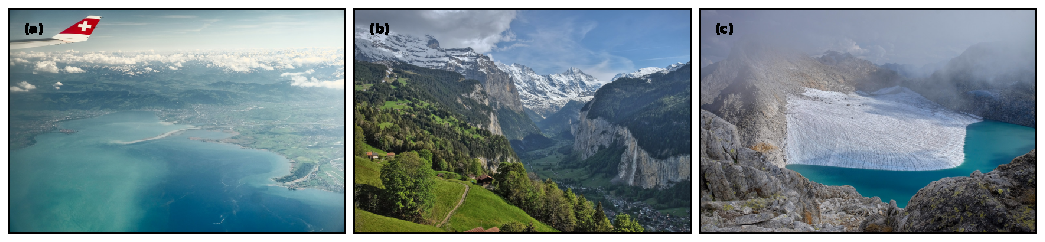
\includegraphics{alpero_landscape}}
      \caption{%
        Alpine glacial erosion landscape diversity.
        \textbf{(a)} Piedmont overdeepening of Lake Constance, ca.~10x50\,km.
        \textbf{(b)} Glacial trough of Lauterbrunnental, ca.~1x10\,km.
        \textbf{(c)} Mountain cirque of Chüebodengletscher, ca.~1x1\,km.}
      \label{fig:landscape}
    \end{figure*}

    \begin{figure*}
      \centerline{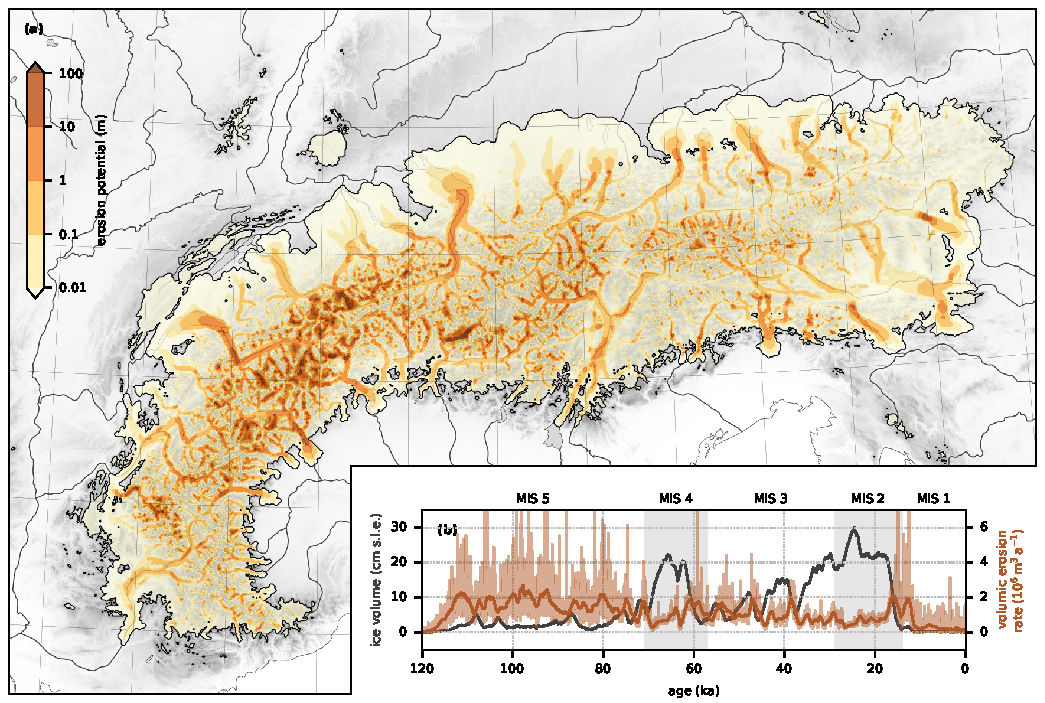
\includegraphics{alpero_cumulative}}
      \caption{%
        \textbf{(a)} Modelled cumulative (time-integrated) glacial erosion
          potential over the last glacial cycle.
        \textbf{(b)} Modelled total ice volume in centimetres of sea-level
          equivalent (cm~s.l.e., black), volumic (domain-integrated) erosion
          rate (light brown) and 100-a running mean (dark brown). Shaded gray
          areas indicate the timing for MIS~2 and~4
          \citep{Lisiecki.Raymo.2005}.} \label{fig:cumulative}
    \end{figure*}

    \begin{figure}
      \centerline{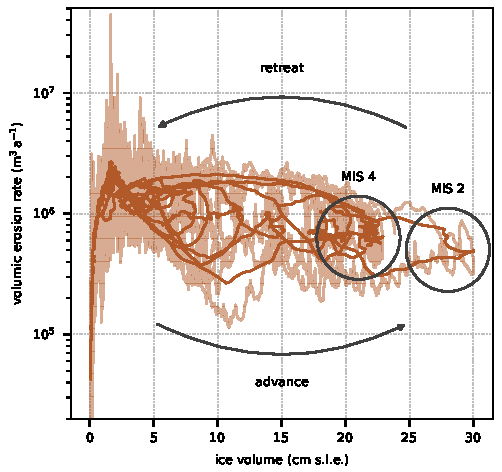
\includegraphics{alpero_evolution}}
      \caption{%
        Modelled volumic (domain-integrated) erosion rate (light brown) and 100-a
        running mean (dark brown) in relation to modelled total ice volume in
        centimetres of sea-level equivalent (black).}
      \label{fig:evolution}
    \end{figure}

    \begin{figure*}
      \centerline{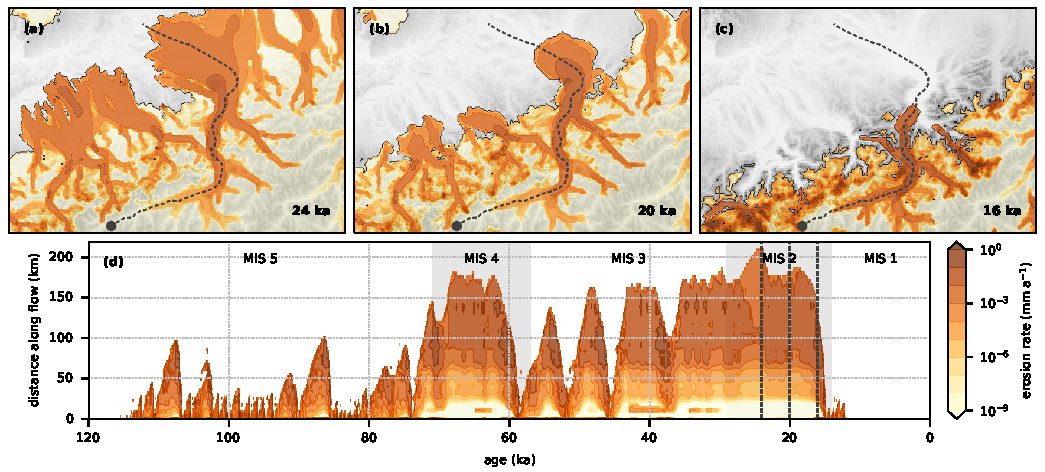
\includegraphics{alpero_transects}}
      \caption{%
        \textbf{(a, b, c)} Modelled instantaneous erosion rate of the Rhine
          Glacier for selected post-Last Glacial Maximum ages.
        \textbf{(d)} Interpolated instantaneous erosion rate along a Rhine
          Glacier transect for the entire last glacial cycle (upper panels
          dashed line).}
      \label{fig:transects}
    \end{figure*}

    \begin{figure*}
      \centerline{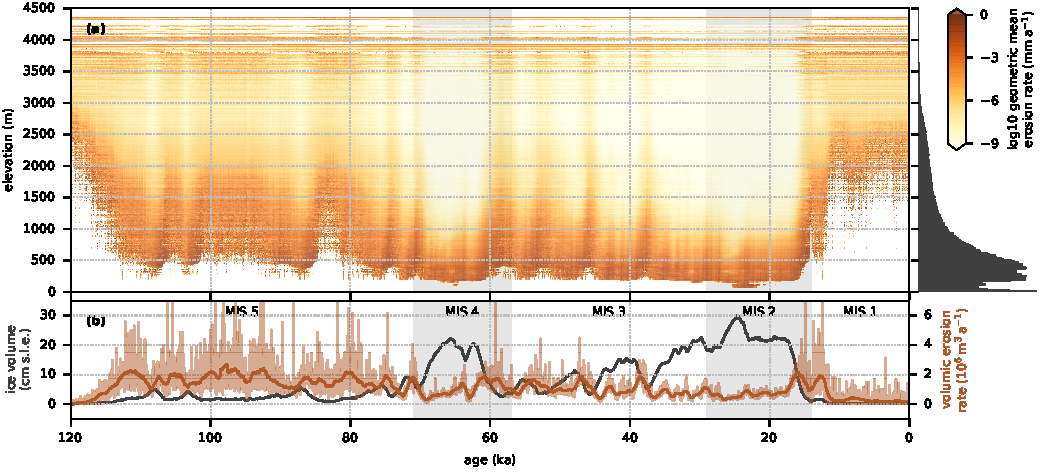
\includegraphics{alpero_hypsogram}}
      \caption{%
        \textbf{(a)} Modelled erosion rate ``hypsogram'', showing the geometric
          mean of (non-zero) modelled erosion rates in 10-m elevation bands
          across the entire model domain and its time evolution.
        \textbf{(b)} Same as Fig.~\ref{fig:cumulative}b.}
      \label{fig:hypsogram}
    \end{figure*}

    \begin{figure*}
      \centerline{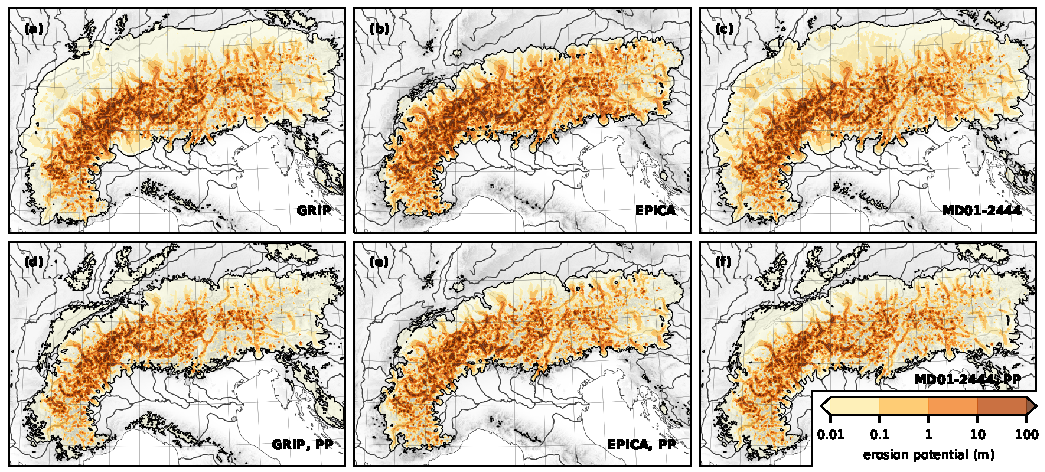
\includegraphics{alpero_sensitivity}}
      \caption{%
        Modelled cumulative glacial erosion potential over the last glacial
        cycle without \textbf{(a, b, c)} and with \textbf{(d, e, f)}
        paleo-precipitation corrections, and using three different
        palaeo-temperature histories \citep[see][]{Seguinot.etal.2018}.}
      \label{fig:sensitivity}
    \end{figure*}

    \begin{figure*}
      \centerline{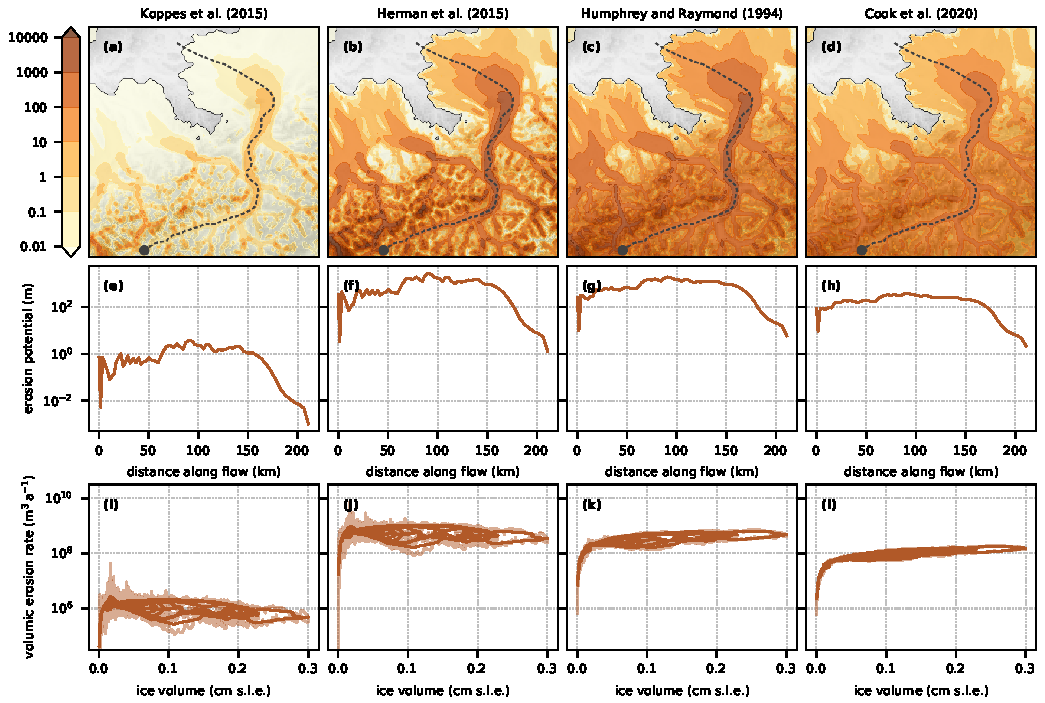
\includegraphics{alpero_powerlaws}}
      \caption{%
        Modelled cumulative (time-integrated) glacial erosion potential for
        three different erosion laws published by
        \textbf{(a)} \citet{Koppes.etal.2015},
          $5.2 \times 10^{-8} u_\mathrm{b} ^{2.34}$ (same as
          Fig.~\ref{fig:cumulative}a but with a different colour scale),
        \textbf{(b)} \citet{Herman.etal.2015},
          $2.7 \times 10^{-7} u_\mathrm{b} ^{2.02}$, and
        \textbf{(c)} \citet{Cook.etal.2020},
          $1.665 \times 10^{-1} u_\mathrm{b} ^{0.6459}$.
        \textbf{(d)} Corresponding erosion power laws, and
        \textbf{(e)} modelled cumulative (time-integrated) glacial erosion
          potential along a Rhine Glacier transect (upper panels dashed line).}
      \label{fig:powerlaws}
    \end{figure*}

% ----------------------------------------------------------------------
% Tables
%\clearpage
% ----------------------------------------------------------------------


% ======================================================================
\end{document}
% ======================================================================
